\documentclass[a4paper]{article}

\usepackage[english]{babel}
\usepackage[utf8]{inputenc}
\usepackage{amsmath}
\usepackage{subfigure}
\usepackage{graphicx}
\usepackage[colorinlistoftodos]{todonotes}
\usepackage{makeidx}
\usepackage{setspace}
\usepackage{float}

\makeindex
\onehalfspacing
\graphicspath{ {images/}{screen/}}

\begin{document}
\begin{titlepage}
	\newcommand{\HRule}{\rule{\linewidth}{0.1 mm}}
	\center
	\textsc{\LARGE Università di Bologna}\\[1.5cm] % Main heading such as the name of your university/college
	
	\HRule\\[0.8 cm]
	{\huge\bfseries Relazione di tirocinio curricolare}\\[0.4cm] % Title of your document
  \HRule\\[1.5cm]
  
	\textsc{\Large Sviluppo e analisi front-end di un prodotto software con workflow
	aziendale}\\[0.3cm] % Main heading such as the name of your university/college
	\textsc{\large Presso Diennea S.R.L}\\[1.5cm] % Main heading such as the name of your university/college
	
	%------------------------------------------------
	%	Author(s)
	%------------------------------------------------
	
	\begin{minipage}{0.4\textwidth}
		\begin{flushleft}
			\large
			\textit{Tirocinante}\\
			\textsc{Matteo Minardi}
		\end{flushleft}
	\end{minipage}
	~
	\begin{minipage}{0.4\textwidth}
		\begin{flushright}
			\large
			\textit{Tutor Aziendale}\\
			\textsc{Enrico Olivelli} % Supervisor's name
    \end{flushright}
    \begin{flushright}
			\large
			\textit{Tutor Didattico}\\
			\textsc{Annalisa Franco} % Supervisor's name
		\end{flushright}
	\end{minipage}
	

	\vfill\vfill\vfill % Position the date 3/4 down the remaining page
  
  {\large Dal \emph{18 Settembre 2017} al \emph{14 Ottobre 2017}}\\[1 cm] % Date, change the \today to a set date if you want to be precise
\end{titlepage}

\section{Introduzione}
\label{sec:Introduzione}

\par L'obiettivo principale di questo tirocinio curricolare era l'inserimento formativo
in un ambiente aziendale con il focus sullo sviluppo e analisi front-end per
migliorare il prodotto aziendale.\\
\par L'azienda ha sede principale a Faenza, è un'azienda di fama internazionale con 
anche una sede estera a Parigi. E' tra le aziende leader nel Digital Marketing 
orientato al Mail Marketing, ha oltre 700 clienti tra cui BMW, Stroili Oro, Ducati,
 Findomestic e molti altri.\\
Diennea è un'azienda che lavora a stretto contatto con i clienti e la loro immagine digitale a 
trecentosessanta gradi. Da quindici anni a questa parte sviluppa un prodotto all'avanguardia
che permette al cliente di gestire tutto ciò che riguarda le campagne pubblicitarie, le newsletter e 
l'interazione digitale con i propri contatti attraverso canali come e-mail e SMS.\\
\par Il mio ruolo in tutto ciò è stato quello di far parte del team \emph{Product\&Care} con il ruolo di 
front-end developer volto a migliorare quelli che sono gli aspetti relativi alla 
veste grafica e alla \emph{UX (User Expirience)} del loro prodotto.\\
Il prodotto in questione ha nome \emph{MagNews}
\begin{figure}[H]
	
\includegraphics[width=4cm]{magnews-diennea.png}
	\centering
\end{figure}
Si occupa di gestire i clienti dell'acquirente all'interno Database su cui vengono
create campagne mirate a pubblicizzarsi nel modo più efficiente, efficace e intelligente 
possibile. Tutto questo è contornato da reportistiche dettagliate, dati in tempo reali 
e moltissime feature interessanti che lo rendono uno dei migliori prodotti in questo
campo in italia.\\ 
E' scontato precisare che per realizzare tutto questo è necessaria la combinazione
di svariate teconlogie che collaborano al fine comune di creare una piattaforma solida
scalabile e resistente allo stress esercitato dall'uso intensivo delle risorse.\\
Le risorse infatti, pur essendo di grossa portata, devono essere usate in modo
performante visto che devono servire milioni di mail ogni giorno e provvedere a centinaia
di migliaia di richieste. Per tutto questo serve un'architettura distribuita moderna 
e scalabile. Ovviamente entrando in un azienda con un alto numero di Developer è 
stato inevitabile affrontare discorsi relativi al versionamento e al workflow aziendale. 
Tutto questo ha concretizzato molte dinamiche viste e affrontate soltanto teoricamente 
durante il percorso accademico. 

\section{Tecnologie}
\label{sec:Tecnologie}
\par In questo tirocinio sono stati toccati tanti argomenti tecnologici moderni
per quanto riguarda l'analisi del framework e, allo stesso tempo, sono stati consolidate
varie tecnologie frontend per lo sviluppo classico. Ora in presenterò un breve elenco
che tocca tutti i punti; ognuno di essi verrà poi analizzato singolarmente quando
parlerò dell'attività di \emph{analisi}.\\
\par Di seguito vengono presentati due elenchi: uno per le tecnologie analizzate e applicate
e uno per le tecnologie utilizzate effettivamente.\\
Tecnologie analizzate:
\begin{itemize}
	\item Angular 2
	\item React JS
	\item Vue JS
\end{itemize}
Tecnologie utilizzate:
\begin{itemize}
	\item HTML, CSS, Javascript
	\item jQuery
	\item Bootstrap
	\item p5.js
	\item Aviary SDK
\end{itemize}
\par Inoltre durante lo sviluppo è sempre stata utilizzata una macchina \emph{Linux Fedora}
in cui si utilizzava il progetto in un repository contenuto localmente in una versione
\emph{on premise} di Atalassian Bitbucket. Questo mi ha permesso di acquisire dimestichezza
con quello che il workflow aziendale per quanto riguarda un progetto.
Tra le tecnologie utilizzate e che verranno dopo osservate vi è anche \emph{Git}.\\
\par Per quanto riguarda il build del prodotto è stato necessario utilizzare un server
\emph{Tomcat} che ospitasse il build dei vari moduli \emph{Maven} presi in considerazione
durante il lavoro.
Per la parte backend sono stati toccati ambiti come:
\begin{itemize}
	\item Maven
	\item Java e JSP
\end{itemize}
\newpage
\section{Attività}
\par In questa sezione verrà illustrata riassuntivamente quella che è stata l'esperienza vera e propria.
Verranno presi in considerazione uno ad uno tutti i task svolti spiegandone il contesto, contestualizzando
ed eventualmente indicandone il monte ore utilizzato.
\subsection{Analisi del framework frontend}
\subsection{Analisi e rework del monitor segnalazioni}
\par Uno dei task di improvement del prodotto più onerosi è stato quello del monitor di controllo.
Internamente hanno un modulo \emph{MagNews} che si occupa della ricezione degli errori,
dei servizi down, dei problemi e molto altro. Essendo una parte interna del prodotto
non è mai stato considerata tutta la parte grafica e \emph{UX}. Con il passare del tempo
il personale che ne fa uso quotidiano ha trovato la necessità di migliorarlo.
Oltre ad un uso interno, ora viene anche fornito al personale addetto delle persone che
lo utilizzano esternamente. Per questi motivi è stato necessario ricorrere ad un restyling
da una situazione di partenza del genere:
\begin{figure}[H]
	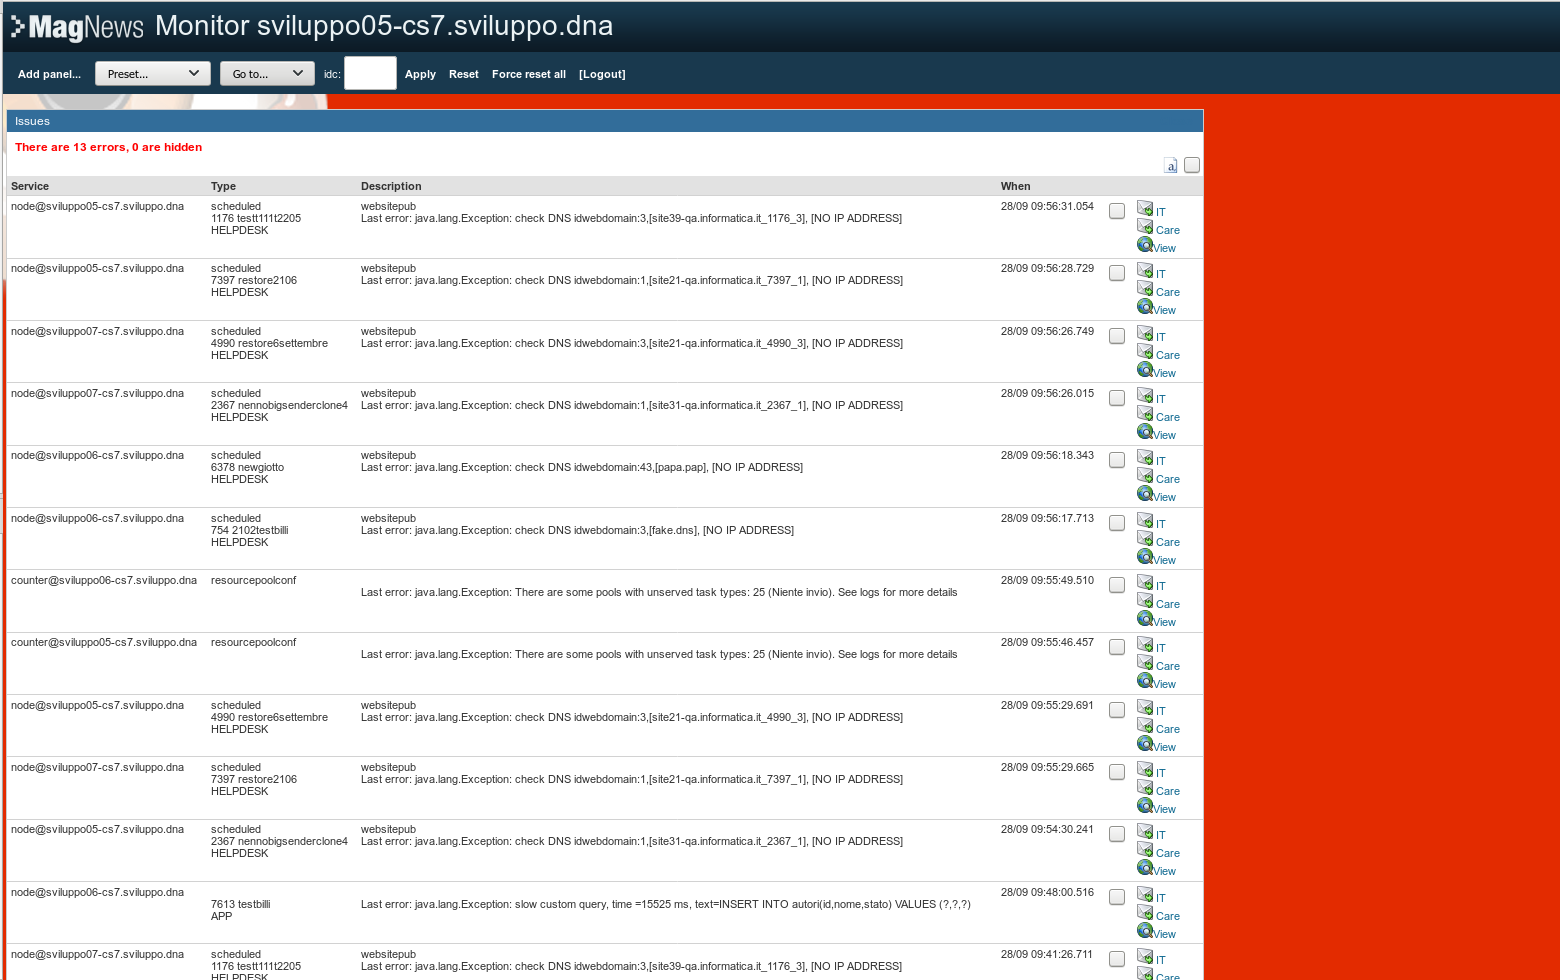
\includegraphics[width=\textwidth]{dashboard_old.png}
	\centering
\end{figure}
In questa figura si può notare che la dasboard è ricca di informazioni, molteplici segnalazioni
ma il contenuto è gestito male, organizzato in modo poco intuitivo e poco gradevole all'utilizzo.
Ogni tabella contiene migliaia di voci disordinate, e ogni pagina può contenere più tabelle
il che rende ancora più confusionario il tutto. Per migliorare tutto questo è stato inserimento
un framework grafico (\emph{Bootstrap}) e una libreria Javascript (\emph{DataTables}) che consentono
di maneggiare al meglio e in modo efficiente i componenti obsoleti utilizzati in precedenza.
Il risultato finale della home è questo:
\begin{figure}[H]
	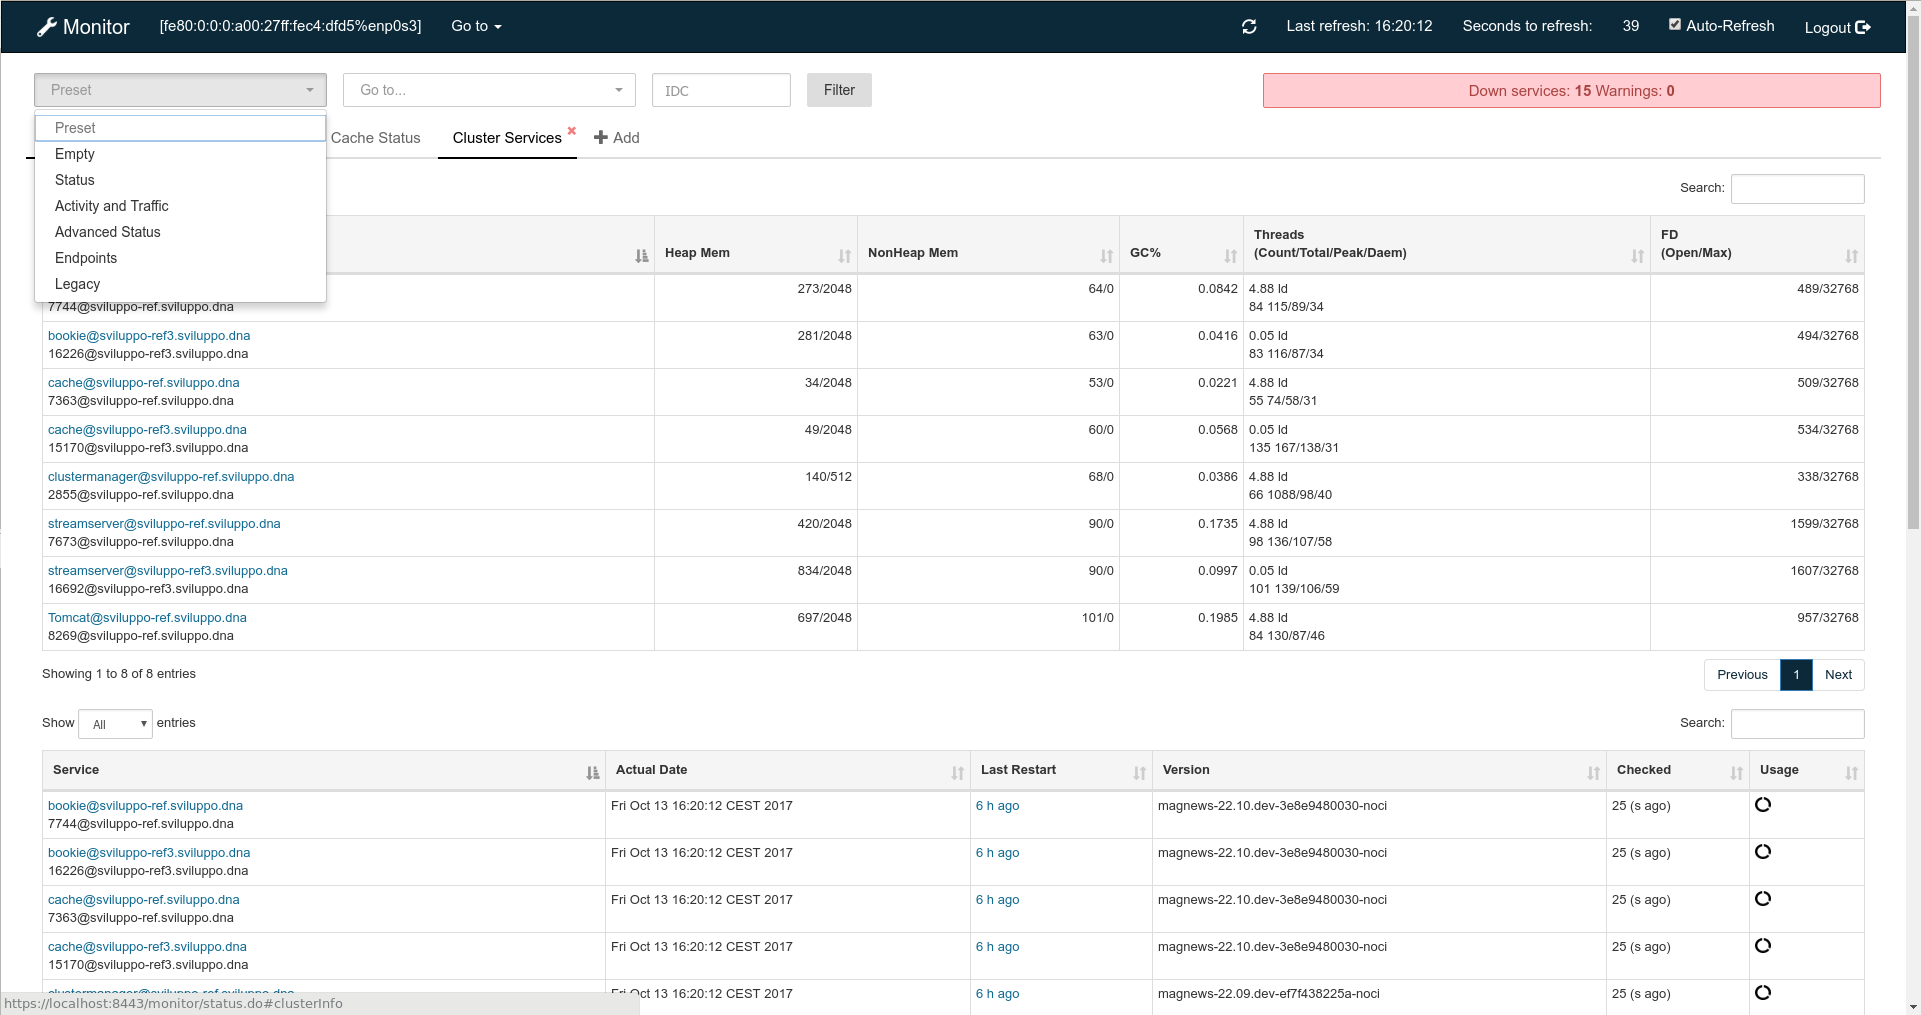
\includegraphics[width=\textwidth]{dashboard_new.png}
	\centering
\end{figure}
La navigazione ad altre pagine è più semplice, l'accesso ai warning e ai downservices
è più agevole e le tabelle sono completamente rinnovate vista l'introduzione della possibilità di
visualizzazione paginata e ordinamento.
\par Oltre ad aver cambiato la dashboard principale ho provveduto a far corrispondere schermate secondarie
che si rifanno allo stesso stile coerente con i colori del brand e l'immagine artistica del prodotto.\\
Per il login:
\begin{figure}[H]
	\centering
	\begin{subfigure}
	  \centering
	  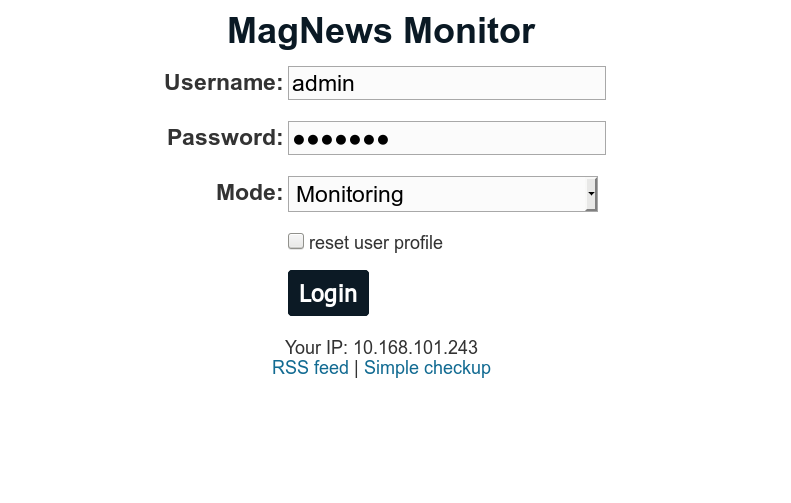
\includegraphics[width=0.45\linewidth]{login_old.png}
	\end{subfigure}%
	\begin{subfigure}
	  \centering
	  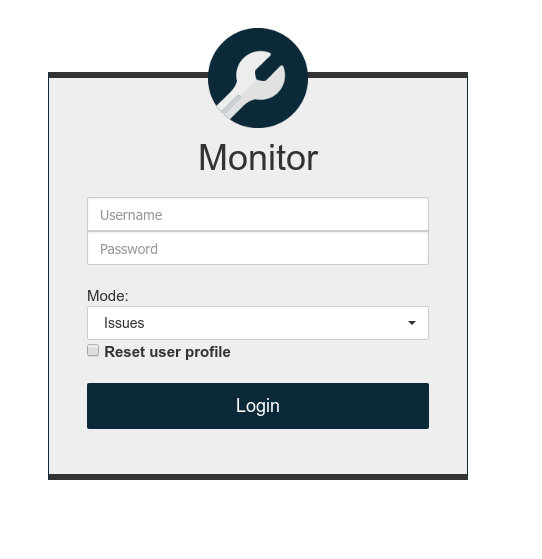
\includegraphics[width=0.45\linewidth]{login_new.png}
	\end{subfigure}
\end{figure}
Per una schermata secondaria fatta in Angular:
\begin{figure}[H]
	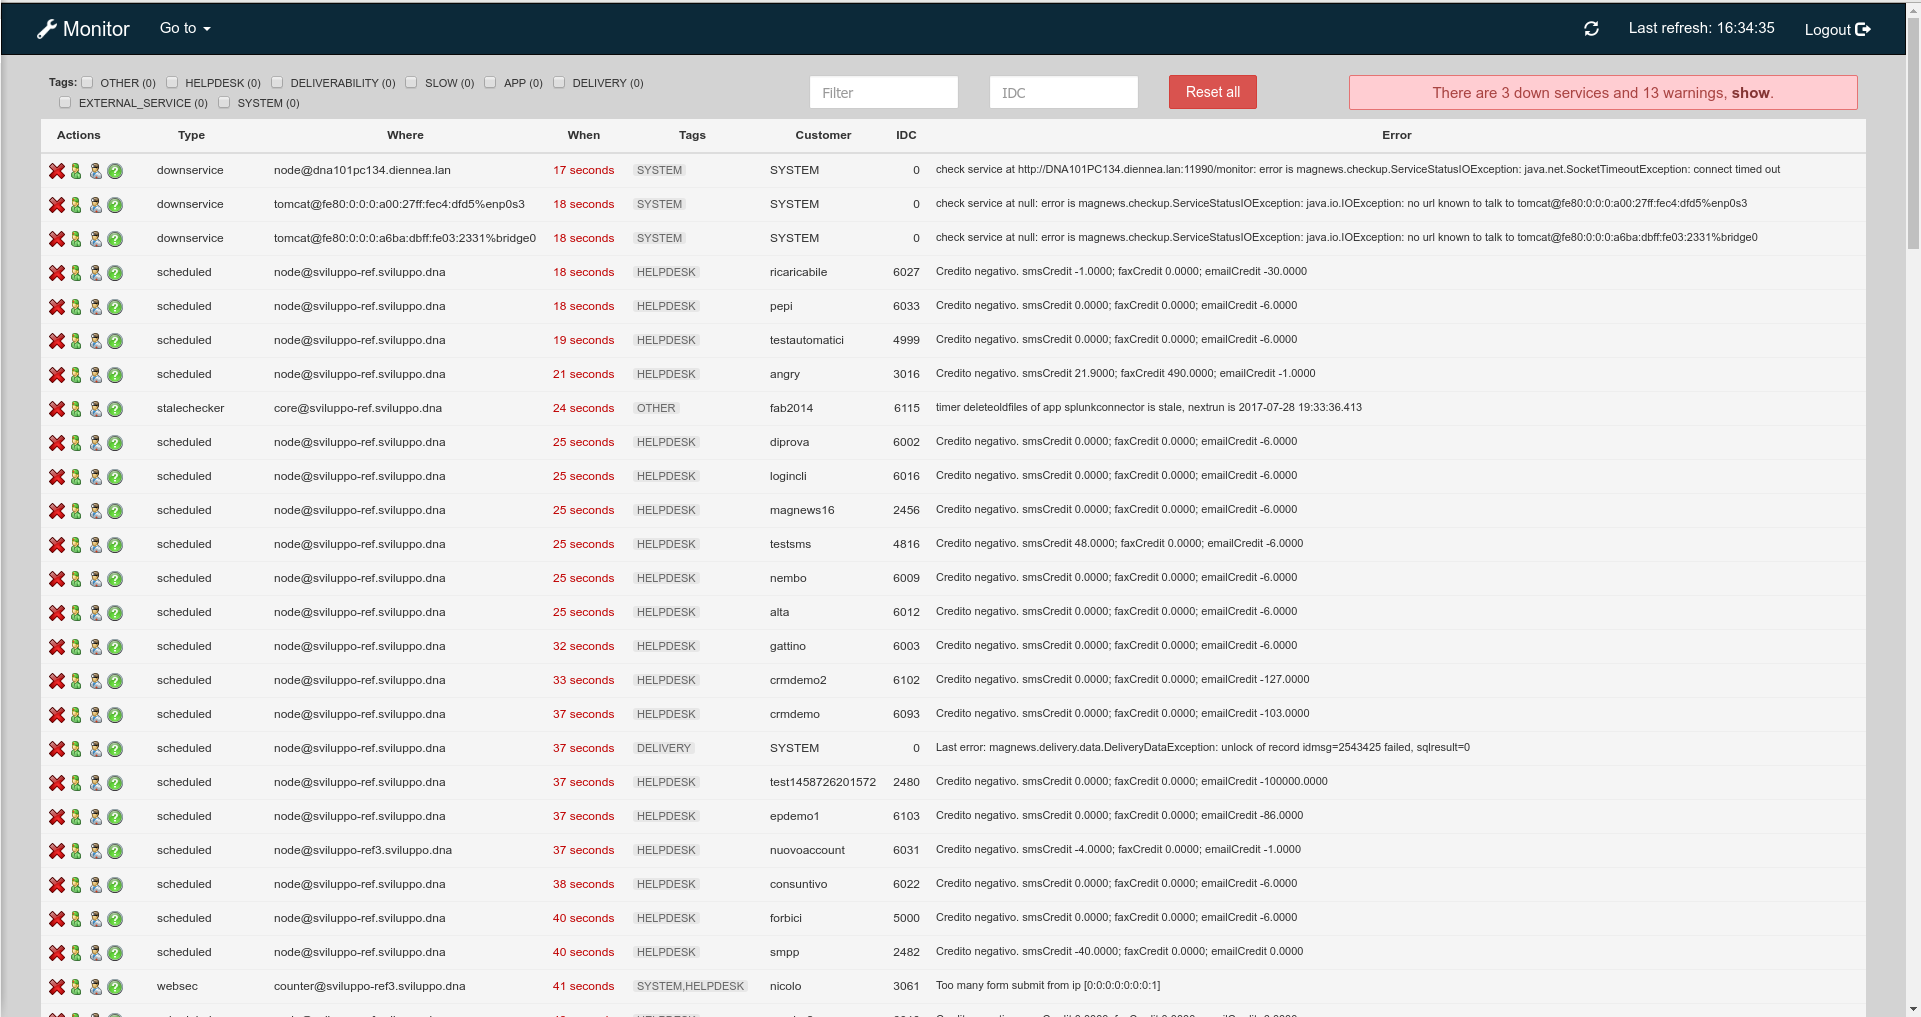
\includegraphics[width=\textwidth]{issue_new.png}
	\centering
\end{figure}
conclusione di questo pezzo
\subsection{Risoluzione issues aziendali}
issue aviary, issue Fly-weight, issue findbugs-spotbugs
\subsection{Rappresentazione grafica delivery}
grafica javascript, API Rest per fare request GET
\subsection{Workflow Git}
Branching, rebasing, workflow

\section{Conclusioni}
\par In conclusione è stata una esperienza nel complesso positiva. Ha avuto alti e bassi in quanto 
a mole di lavoro e produttività. Nei momenti lati includerei la grande quantità
di esperienza acquisita a contatto con senior developers, esperienza di quella che è
la modalità di lavoro in collaborazione e la vasta copertura tecnologica all'interno
dell'azienda. Nei lati negativi inserirei assolutamente la difficoltà in un tirocinio
di 150 ore ad inserirsi in un progetto di quella complessità riuscendo ad avere un 
impatto vero e proprio. \\
Questo tipo di esperienza ti apre gli occhi sul mondo del lavoro ma allo stesso tempo
ti fa realizzare che in ambito informatico l'orizzonte è ampio e c'è una vasta disomogeneità
su quella che è la conoscenza richiesta.
\renewcommand{\refname}{Bibliografia}
\begin{thebibliography}{9}
  \bibitem{latexcompanion} 
  Michel Goossens, Frank Mittelbach, and Alexander Samarin. 
  \textit{The \LaTeX\ Companion}. 
  Addison-Wesley, Reading, Massachusetts, 1993.
   
  \bibitem{einstein} 
  Albert Einstein. 
  \textit{Zur Elektrodynamik bewegter K{\"o}rper}. (German) 
  [\textit{On the electrodynamics of moving bodies}]. 
  Annalen der Physik, 322(10):891–921, 1905.
   
  \bibitem{knuthwebsite} 
  Knuth: Computers and Typesetting,
  \\\texttt{http://www-cs-faculty.stanford.edu/\~{}uno/abcde.html}
  \end{thebibliography}

\end{document}